\subsection{Data Collection}
\subsubsection{Data Sources}
Collecting data from diverse e-commerce platforms ensures a broad and comprehensive dataset. This diversity helps in creating more generalized models that can handle various types of product descriptions and specifications.

\subsubsection{Data Format}
JSON format is chosen for its versatility and compatibility with modern web technologies. JSON allows for easy manipulation and querying of data, making it a preferred choice for data scientists and engineers.

\subsubsection{Data Cleaning Process}
Cleaning the data is essential to remove any inconsistencies that could affect the model's performance. This involves:

\begin{itemize}
    \item \textbf{Duplicate Removal:} Ensuring that no redundant data skews the training process.
    \item \textbf{Normalization:} Standardizing the data entries so that they follow a uniform structure.
    \item \textbf{Format Conversion:} Converting all data entries into a consistent format, such as JSON, ensures that the data can be easily processed and fed into the models.
\end{itemize}

\subsection{Data Preparation}
\subsubsection{Data Normalization}
This step ensures that all product entries are consistent, which is crucial for training the models effectively. Normalization involves standardizing units of measurement, converting text to a common case, and ensuring that similar attributes are grouped together.

\subsubsection{Data Structuring}
Proper structuring of data is vital for efficient model training. This involves organizing the data into categories and subcategories, making it easier for the models to understand and learn from the data.

\subsection{Model Fine-Tuning}
\subsubsection{Hyperparameter Selection}
Finding the right hyperparameters is a critical part of the fine-tuning process. Hyperparameters are settings used to control the training process, such as learning rate, batch size, and the number of training epochs. Selecting optimal hyperparameters helps in achieving better model performance.

\subsubsection{Optimization Methods}
Using advanced optimization techniques, such as gradient descent, helps in fine-tuning the pre-trained weights of the models. This process involves adjusting the model parameters to minimize the error between the predicted and actual outputs.

\subsubsection{JSON-Tuning}
A novel approach that leverages structured data in JSON format to enhance the performance of LLMs. This technique improves the models' ability to generate accurate and contextually relevant reviews by providing them with well-organized and structured data.

\subsection{Model Evaluation}
\subsubsection{BLEU}
This metric measures the precision of the generated reviews by comparing them with reference translations. Higher BLEU scores indicate better alignment with human-generated references.

\subsubsection{ROUGE}
This metric evaluates the overlap between the generated reviews and reference texts. It focuses on recall, measuring how much of the reference text is captured in the generated output.

\subsubsection{METEOR}
This metric considers various matching techniques, including synonymy and stemming, to evaluate the alignment between the generated and reference texts. It provides a more nuanced evaluation by considering semantic similarities.

\subsection{Results Analysis}
The final step involves analyzing the results obtained from the model evaluation. This includes assessing:

\begin{itemize}
    \item \textbf{Accuracy:} How closely the generated reviews match the reference texts in terms of content and meaning.
    \item \textbf{Fluency:} The readability and coherence of the generated reviews. High fluency indicates that the reviews are not only accurate but also easy to read and understand.
    \item \textbf{Relevance:} The extent to which the generated reviews are pertinent to the product being described. This ensures that the reviews provide valuable insights to potential customers.
    \item \textbf{Hallucinations:} Instances where the models generate content that is factually incorrect or irrelevant. Minimizing hallucinations is crucial for maintaining the credibility and usefulness of the generated reviews.
\end{itemize}

\begin{figure}[H]
    \centering
    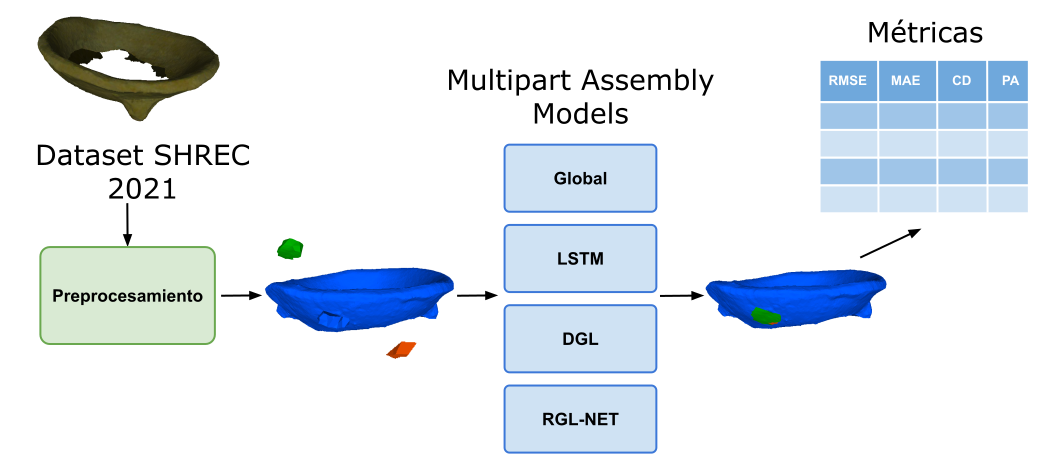
\includegraphics[width=12cm]{images/Methodology.jpg}
    \caption{Methodology Flowchart}
    \label{fig:MethodologyFlowchart}
\end{figure}